\documentclass[tikz,border=10pt]{standalone}
\usetikzlibrary{matrix,shapes.geometric}

\tikzset{
  mybox/.style={
    draw,
    rectangle,
    rounded corners,
    minimum width=3cm,
    minimum height=3cm,
    text centered,
    font=\small
  }
}

\begin{document}
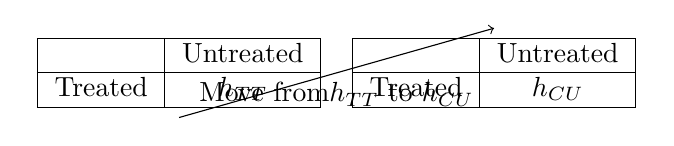
\begin{tikzpicture}
  % Left Panel (All Treated)
  \node (leftPanel) at (0,0) {
    \begin{tabular}{|c|c|}
      \hline
      & Untreated \\
      \hline
      Treated & $h_{TT}$ \\
      \hline
    \end{tabular}
  };
  
  % Right Panel (All Untreated)
  \node (rightPanel) at (4,0) {
    \begin{tabular}{|c|c|}
      \hline
      & Untreated \\
      \hline
      Treated & $h_{CU}$ \\
      \hline
    \end{tabular}
  };

  % Arrows between Panels
  \draw[->] (leftPanel.south) -- node[midway, below] {Move from \\ $h_{TT}$ to $h_{CU}$} (rightPanel.north);
\end{tikzpicture}
\end{document}